\section{Price analysis}\label{Sec:Price analysis}

One of the core factors in the choice of the property to book is its price, being one of main drivers of customers' behaviors \citep{liang2018understanding}. Therefore one may want to try and see what properties' attributes influence its value.

We start in subsection \ref{subsec:corr} by calculating the correlation of all the other variables with respect to price. Then we try in subsection \ref{subsec:lm} to run a linear regression on price to look what variables are statistically relevant and how much they affect the price.


\subsection{Correlation with price}\label{subsec:corr}

Since we are only interested in the correlation with price, a classic correlation plot like the one produced by \texttt{corrplot} from the package \texttt{corrplot} may not be the most easily readable in this case, especially because of the large number of variables.

In fact, categorical variables first need to be transformed into many dummy variables in order to calculate the correlation. The function \texttt{from\_row\_to\_col} will be used to achieve this result. It creates dummy variables for all factor levels by creating a column of 1s, spreading it across so many columns as factor levels and filling the empty rows in the columns with 0s.

\lstinputlisting[language=R, firstline=2, escapechar=|, caption={|\textbf{\href{https://github.com/silvia-ventoruzzo/SPL-WISE-2018/blob/master/Helpers/from_row_to_col.R}{from\_row\_to\_col.R}}|}]{../Helpers/from_row_to_col.R}


\begin{figure}[H]
\begin{center}
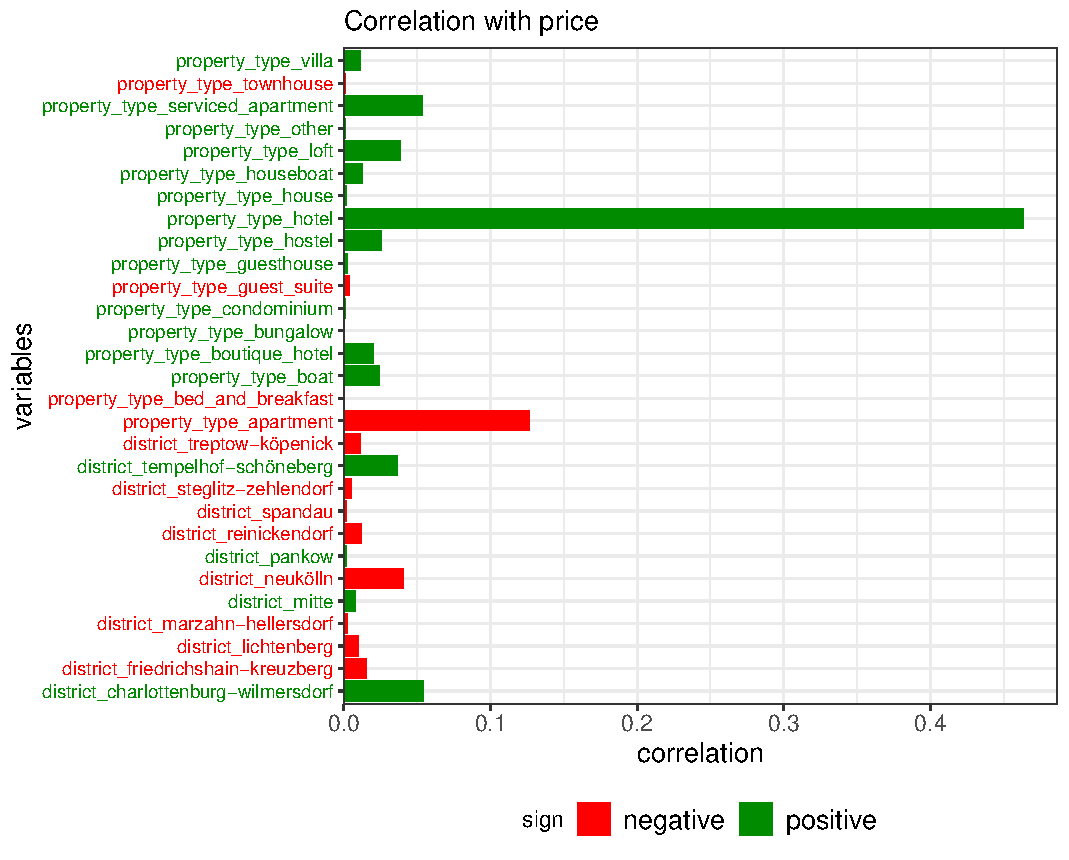
\includegraphics[width=0.8\textwidth, keepaspectratio]{price_correlation.pdf} \\
\caption{Sample of plot of correlation with price \protect
\includegraphics[scale=0.05]{qletlogo.pdf} {\href{https://github.com/silvia-ventoruzzo/SPL-WISE-2018/blob/master/Helpers/correlation_plot.R}{correlation\_plot.R}}}
\label{figure:pricecorr}
\end{center}
\end{figure}



\subsection{Linear regression on price}\label{subsec:lm}

As pointed out in \cite{wang2017price} linear regression is used to describe possible linear relationships between a dependent variable and one or multiple independent variables.

In this case we will look for the relationship that the properties' attributes have on their price. For this purpose we used again the data with the categorical variables transformed to dummies. The linear regression was then run using all other variables, except \textit{id}, \textit{long}, \textit{lat}, \textit{neighbourhood} and \textit{listing\_url}, as regressors.

On table \ref{table:lmresults} you can see a sample of the results. A positive coefficient means that the variable has a positive impact on the dependent variable, the higher this regressor is, the higher \textit{price} will be. On the other side, a negative coefficient suggests that a higher value of the independent variable will result in a lower value of \textit{price}. Moreover, a variable is considered significant if the p-value is lower than the significance level, set at 5\% in this case, since it rejects the null hypothesis for that regressor coefficient to be equal to zero \citep{moye2006statistical}.

\begin{table}[H]
\centering
\begin{tabular}{lrl}
  \hline
variable & coefficient & significant \\ 
  \hline
(Intercept) & 12.69 & FALSE \\ 
  host\_listings\_count & -0.73 & TRUE \\ 
  accommodates & 16.31 & TRUE \\ 
   \hline
\end{tabular}
\caption{Sample of linear regression results}
\label{table:lmresults}
\end{table}

Furthermore, to check the validity of the model one should also look at the distribution of the residuals, which should be normal. One can see from table \ref{table:lmresidualst} and picture \ref{figure:regrplots} that this is here not the case.

\begin{table}[H]
\centering
\begin{tabular}{rrrrrrrr}
  \hline
min & 1Q & median & 3Q & max & iqr & mean & sd \\ 
  \hline
-947.97 & -18.72 & -3.31 & 12.32 & 8625.31 & 31.04 & 0.00 & 138.02 \\ 
   \hline
\end{tabular}
\caption{Descriptive statistics of regression residuals}
\label{table:lmresidualst}
\end{table}

\begin{figure}[H]
\centering
\subfloat[Fitted vs. Actual Plot]{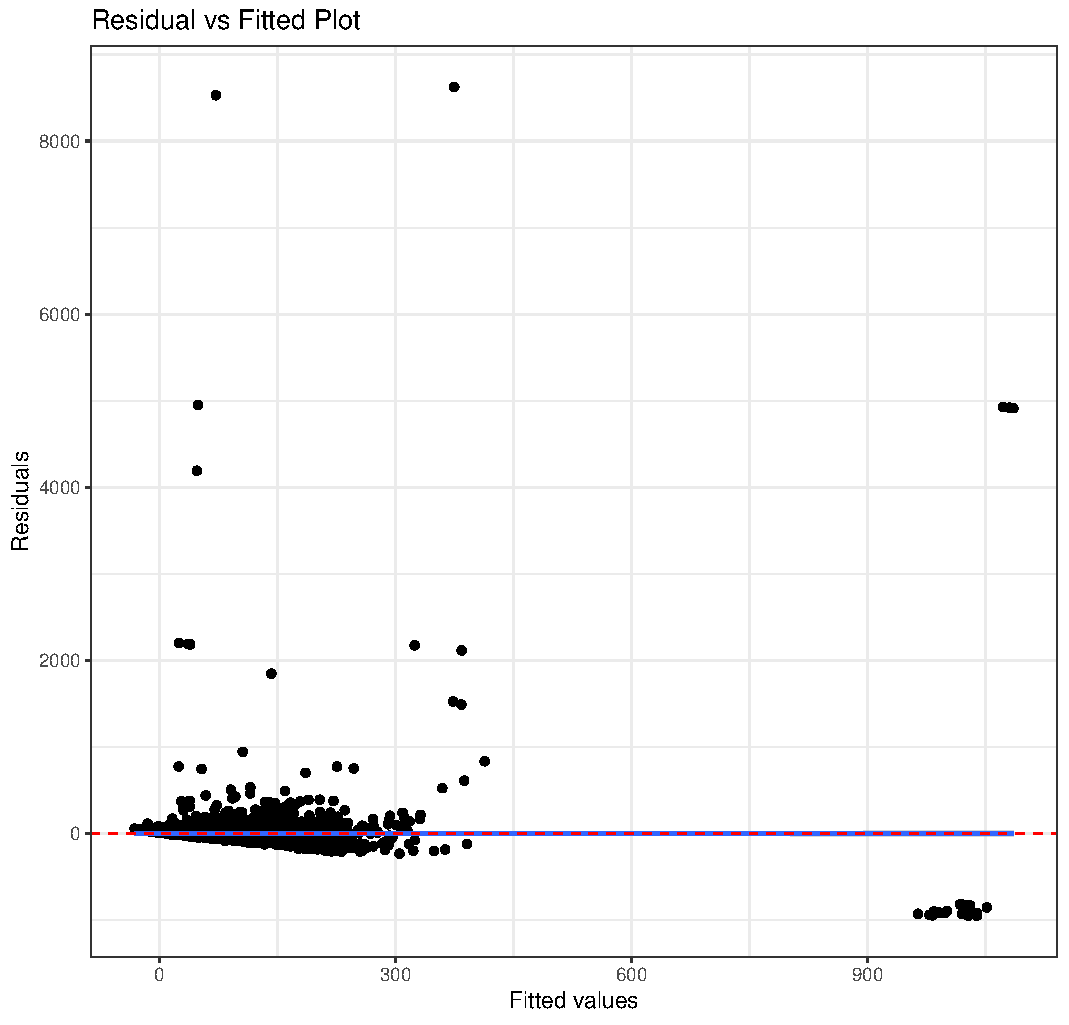
\includegraphics[height=0.5\textwidth]{fittedactual.pdf}}
\subfloat[Residuals QQ Plot]{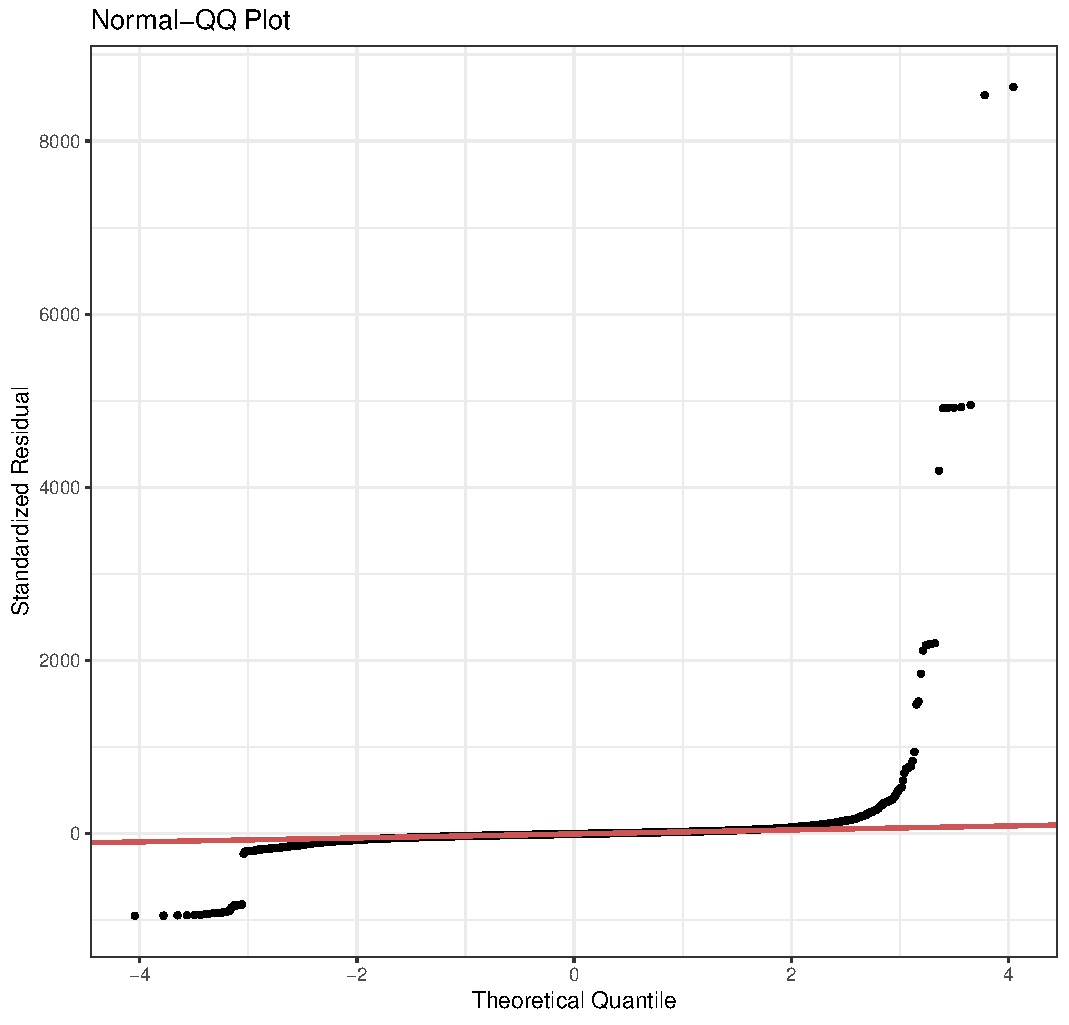
\includegraphics[height=0.5\textwidth]{qqplot.pdf}
\label{figure:cluster_plot}}
\caption{Plotting the clusters}
\label{figure:regrplots}
\centering
\end{figure}

Finally, the $R^2$ for this model, that is the proportion of the variance of \textit{price} captured by the regressors, is only 0.1298, meaning that there is much room for improvement. One can test linear regression with other variables using the ShinyApp described in \ref{Sec:shiny}.